\documentclass[12pt,a4paper, doc]{apa7}

\usepackage[british]{babel}

\usepackage{lscape}
\usepackage{csquotes} 
\usepackage[style=apa]{biblatex}
\DeclareLanguageMapping{british}{british-apa} 
\addbibresource{references.bib} 
% Formatting
\usepackage{setspace} % For line spacing
\doublespacing         % APA recommends 1.5 or double spacing
\usepackage{mathptmx}
\usepackage{graphicx}
\usepackage{float}
\graphicspath{ {./Content/Figures/} } % For figures
\usepackage{caption}
\usepackage{subcaption}

% Titles
\usepackage{titlesec}

\setcounter{secnumdepth}{4}

\titleformat{\paragraph}
{\normalfont\normalsize\bfseries}{\theparagraph}{1em}{}
\titlespacing*{\paragraph}
{0pt}{3.25ex plus 1ex minus .2ex}{1.5ex plus .2ex}

% Tables
\usepackage{ltablex, booktabs, ragged2e, setspace, float, caption}
\keepXColumns
\newcolumntype{L}[1]{>{\RaggedRight\arraybackslash}p{#1}} 
\newcolumntype{Y}{>{\RaggedRight\arraybackslash}X}
\sloppy



% Title and Author
\title{Value for money Resilience: Nature-Based Solutions for New Zealand’s Urban Transport Networks}
\shorttitle{NbS for Urban Transport Resilience}

\author{Lucy Dunshea}
\affiliation{University of Canterbury}
\course{GEOG695 - Thesis}

\leftheader{Dunshea}

% Abstract
\abstract{Coastal urban environments are increasingly vulnerable to the impacts of flooding, driven by both climatic factors—such as sea-level rise and extreme rainfall—and anthropogenic influences, including land use changes and urban densification. In New Zealand, floods are the most frequent and second most costly natural disaster, following earthquakes. Global projections estimate that flood-related economic losses will continue to rise unless adaptive strategies are implemented. Nature-Based Solutions (NBS) have emerged as a promising umbrella framework for addressing both environmental and societal challenges using naturally occurring systems and processes. Within the urban water management context, sub-frameworks such as Water-Sensitive Urban Design (WSUD), Green-Blue Infrastructure (GBI), Low Impact Development (LID), and Sustainable Urban Drainage Systems (SUDS) offer practical strategies to mitigate flood risks while delivering co-benefits for communities.}

\keywords{Nature-based solutions, transport resilience, flooding, green infrastructure, Petone}

\begin{document}

\maketitle
\newpage

%================== BODY ==================%
\section{Acknowledgements}
\section{Abstract}

\newpage
\tableofcontents
\newpage
\section{Introduction}
\subsection{Background}

\begin{landscape}
\begin{figure}
    \centering
    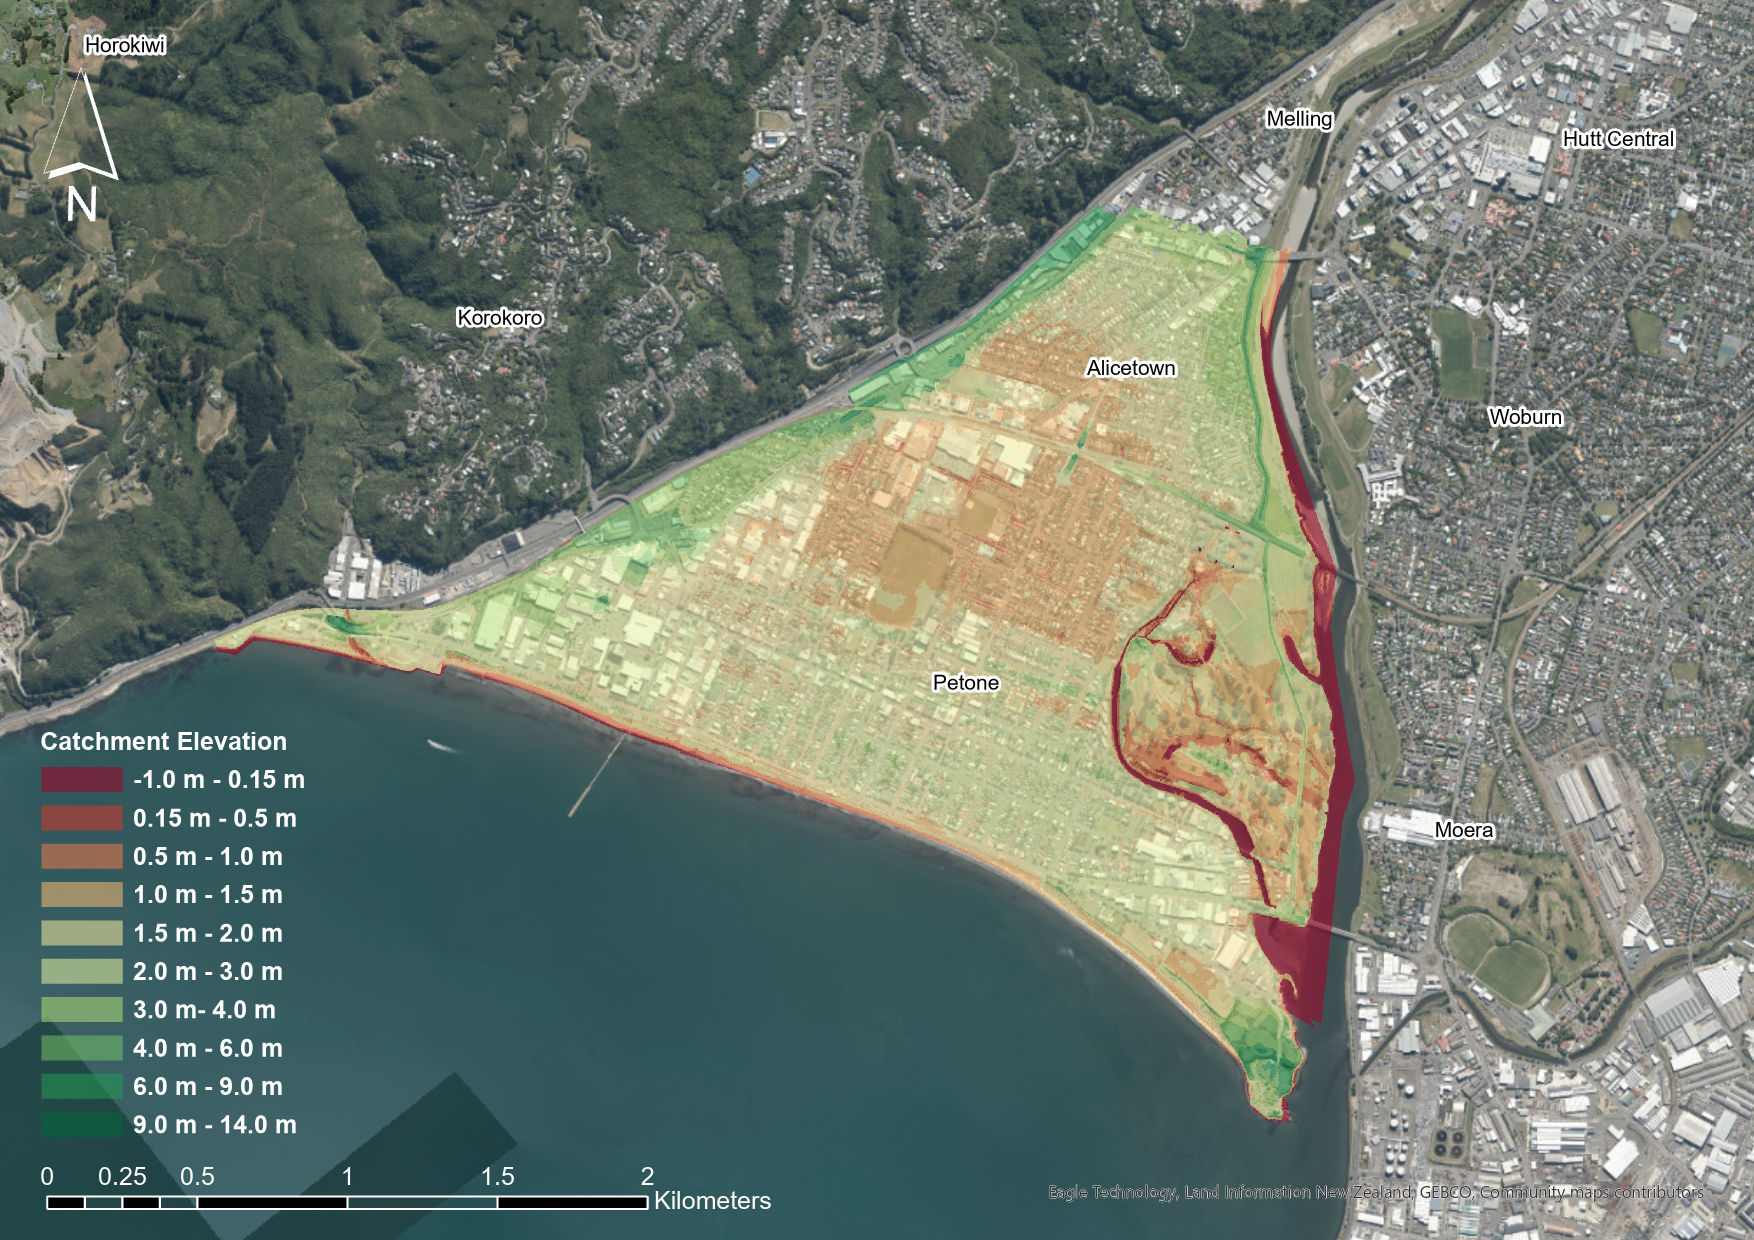
\includegraphics[width=1.0\linewidth]{Content/Figures/01_Introduction/Elevation-map.pdf}
    \caption{Elevation of Petone}
    \label{fig:elevation-map}
\end{figure}
\end{landscape}

\subsubsection{Case Study Area}

\begin{figure}
    \centering
    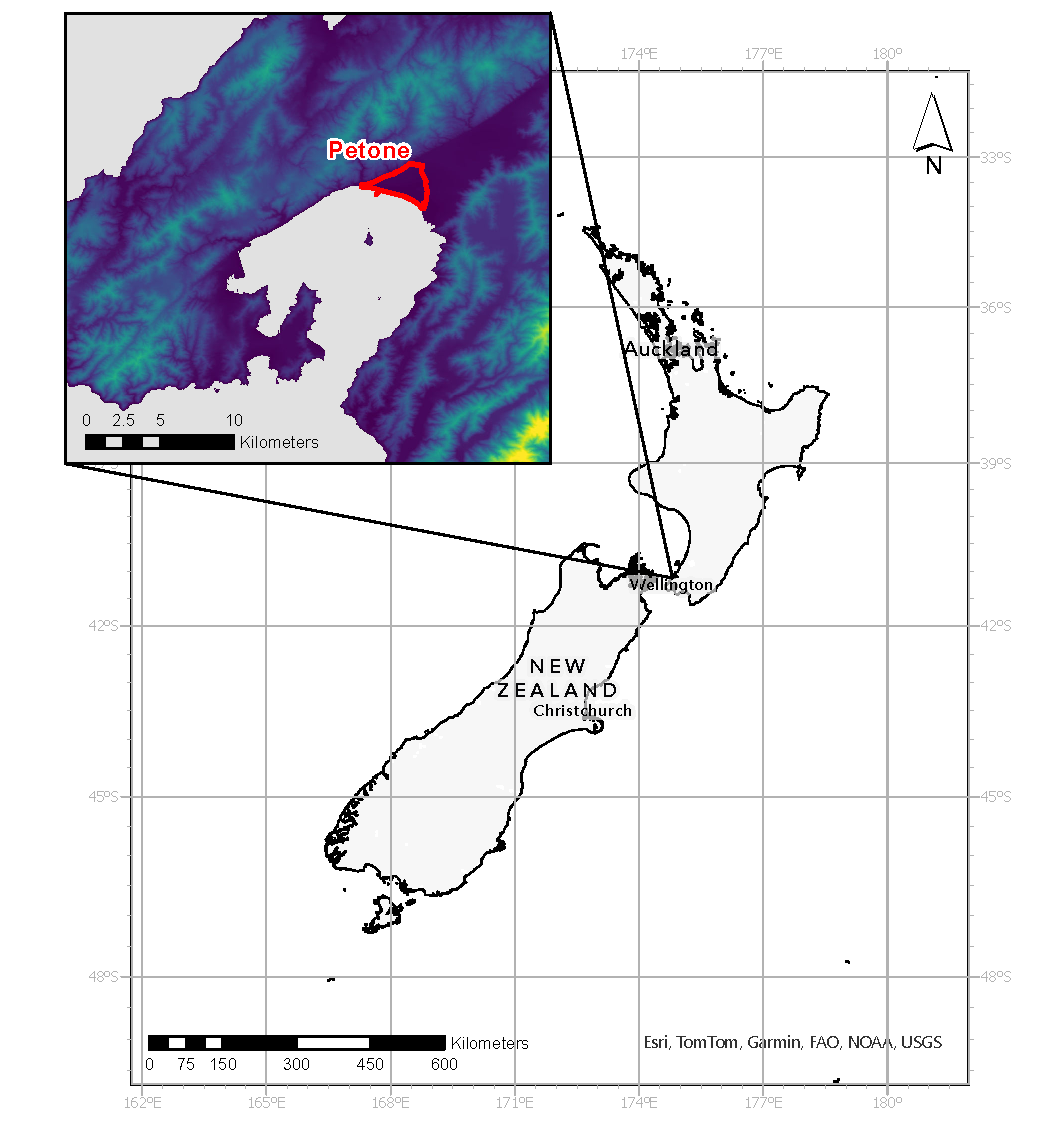
\includegraphics[width=1.0\linewidth]{Content/Figures/01_Introduction/study-area.pdf}
    \caption{Caption}
    \label{fig:enter-label}
\end{figure}

\subsection{Research Question}
\subsubsection{Research Objectives}
\begin{itemize}
    \item To identify which critical transport assets within the Petone-Alicetown catchment are vulnerable to flooding (coastal inundation, pluvial, fluvial) under current and future sea-level rise and climate scenarios as identified in the IPCC sixth assessment report and downscaled by NIWA (Andrews, 2023).
    \item To design and evaluate the technical feasibility of selected adaptation scenarios which highlight the use of NbS for addressing both coastal inundation and flooding from extreme rainfall compared to traditional grey infrastructure approaches, and to consider their role in a longer-term retreat strategy for Petone.
    \item To examine the cost-effectiveness of the selected adaptation options given the regulatory, financial, and governance barriers to their implementation within Hutt City’s existing urban transport system.
    \item To consider how the implementation of larger proposed transport projects (Cross Valley Link, River Link, Petone to Grenada) may: 
\begin{itemize}
    \item Alter the adaptation needs for the Petone-Alicetown catchment, and
    \item Be integrated with NbS adaptation options.
\end{itemize}
\end{itemize}




\subsection{Thesis Outline}


\section{Literature Review}
\subsection{Flood Risk}
Flooding is one of the world’s most pervasive natural hazards, with
approximately 1.47 billion people, or 19 percent of the world’s population,
directly exposed to significant risks during 1-in-100-year flood events
\parencite{IPCC2023}. The strategic benefits of settling near the coast,
including the ease of trade, access to food and other resources, and simply its
unique sense of place has meant that globally approximately 896 million people
live in low-lying coastal areas. However, accelerating urbanisation rates in
areas predisposed to flood risks combined with a changing climate means that
major coastal cities, including New York, Jakarta, Dhaka, and Amsterdam, are
experiencing increased flood vulnerability \parencite{Caljouw2009, Haque2010,
Kim2019, Madajewicz2020}. Even with significant advances in flood management
technology, it is claimed that humanity is more exposed to flood risk today than
ever before \parencite{White2013}.

This trend of growing exposure is no different in New Zealand, where a major
flood occurs every four months on average, each resulting in average damage
costs of \$2 million NZD, for the last 40 years \parencite{CrawfordFlett2022}.
\textcite{Paulik2023} estimated that 441,384 residential buildings are exposed
to flood hazards in New Zealand, with a replacement value of approximately NZD
\$218 billion, a figure that continues to grow despite increasing knowledge of
the exposure to flood risk throughout the country \parencite{Levy2023,
Naish2024, Paulik2023, Hughes2015}. As sea levels rise and the severity of
extreme rainfall events increases \parencite{MfE2023}, coastal developments are
increasingly exposed to more frequent and severe natural hazards, including
inundation, erosion and shoreline recession \parencite{Storey2024}. Strategies
to manage this growing risk in New Zealand are becoming more integrated into
policy and decision-making practices \parencite{Schneider2020, Storey2024,
Storey2025}, however the reality of responding to flood risk in existing coastal
urban areas is that a highly complex and nuanced approach is required to ensure
an equitable transition to a resilient future \parencite{Hughes2015, Logan2020} 

This chapter evaluates the existing research identifying flooding as a core
threat to the function of urban communities situated in the coastal zone
\parencite{Fu2023, kool2020, Pennington2025, Schneider2020, White2013}. It
begins by defining flooding, its sources, and its primary climatic and
anthropogenic drivers, then focuses on the hazard terminology used to describe
flood risk in the context of community resilience. The distinctive patterns and
processes which contribute to flood risk in New Zealand’s coastal settlements
will then be discussed. It also examines how floods are predicted and how the
uncertainty associated with these predictions is managed. Finally, the emerging
paradigm shift from technocentric flood management towards resilient,
nature-based approaches is introduced \parencite{White2013}. A clear
understanding of the risk which flooding poses to communities allows for the
development of adaptive management practices for coastal urban areas like
Petone.

\subsubsection{Defining Flooding}
The first challenge of responding to flooding in urban areas is understanding
the subjective nature of the phenomenon. As \textcite{Pennington2025} explains,
the phrase 'fixing flooding' can refer to addressing minor nuisance flooding on
a private property, or much more convoluted strategies, such as the relocation
of Indonesia’s entire capital city from the subsiding, flood-prone Jakarta to
Nusantara \parencite{Perwira2024}. Ultimately, how flooding is defined shapes
the design of flood adaptation policies \parencite{Schneider2020}, placing
importance on clearly identifying the nature and severity of flood risk present
in a given area, such as the Petone-Alicetown catchment.

Assessing and responding to floods is the domain of multiple disciplines,
including hydrology, sociology, economics, geography, and environmental science
\parencite{Solin2013}. Differing priorities of each discipline have resulted in
varying definitions of the term ‘flood’ within the literature \parencite{Fu2023,
Pennington2025, Ward1978, White2013, WMO2011}. However, a practical definition
of flooding used in hydrology, concerned with the study of the volume, storage,
and movement of water within the earth’s system \parencite{Salas2014} (see
figure~\ref{fig:hydrocycle}), is given by the World Meteorological Organisation:
‘the, usually brief, rise in water level of a stream or water body to a peak
from which the water level recedes at a slower rate.’ \parencite{WMO2011}. This
simplistic definition recognises that flooding is periodical in its nature and
can be considered a naturally occurring state of a water body, akin to drought
conditions \parencite{White2013}. The lack of a single quantitative value also
emphasises that flood levels are catchment specific \parencite{Pennington2025}.
Although this definition is helpful to contextualise flooding within the
hydrological cycle, a different framing of the concept is required to understand
its impacts on people and society.

\begin{figure}
\centering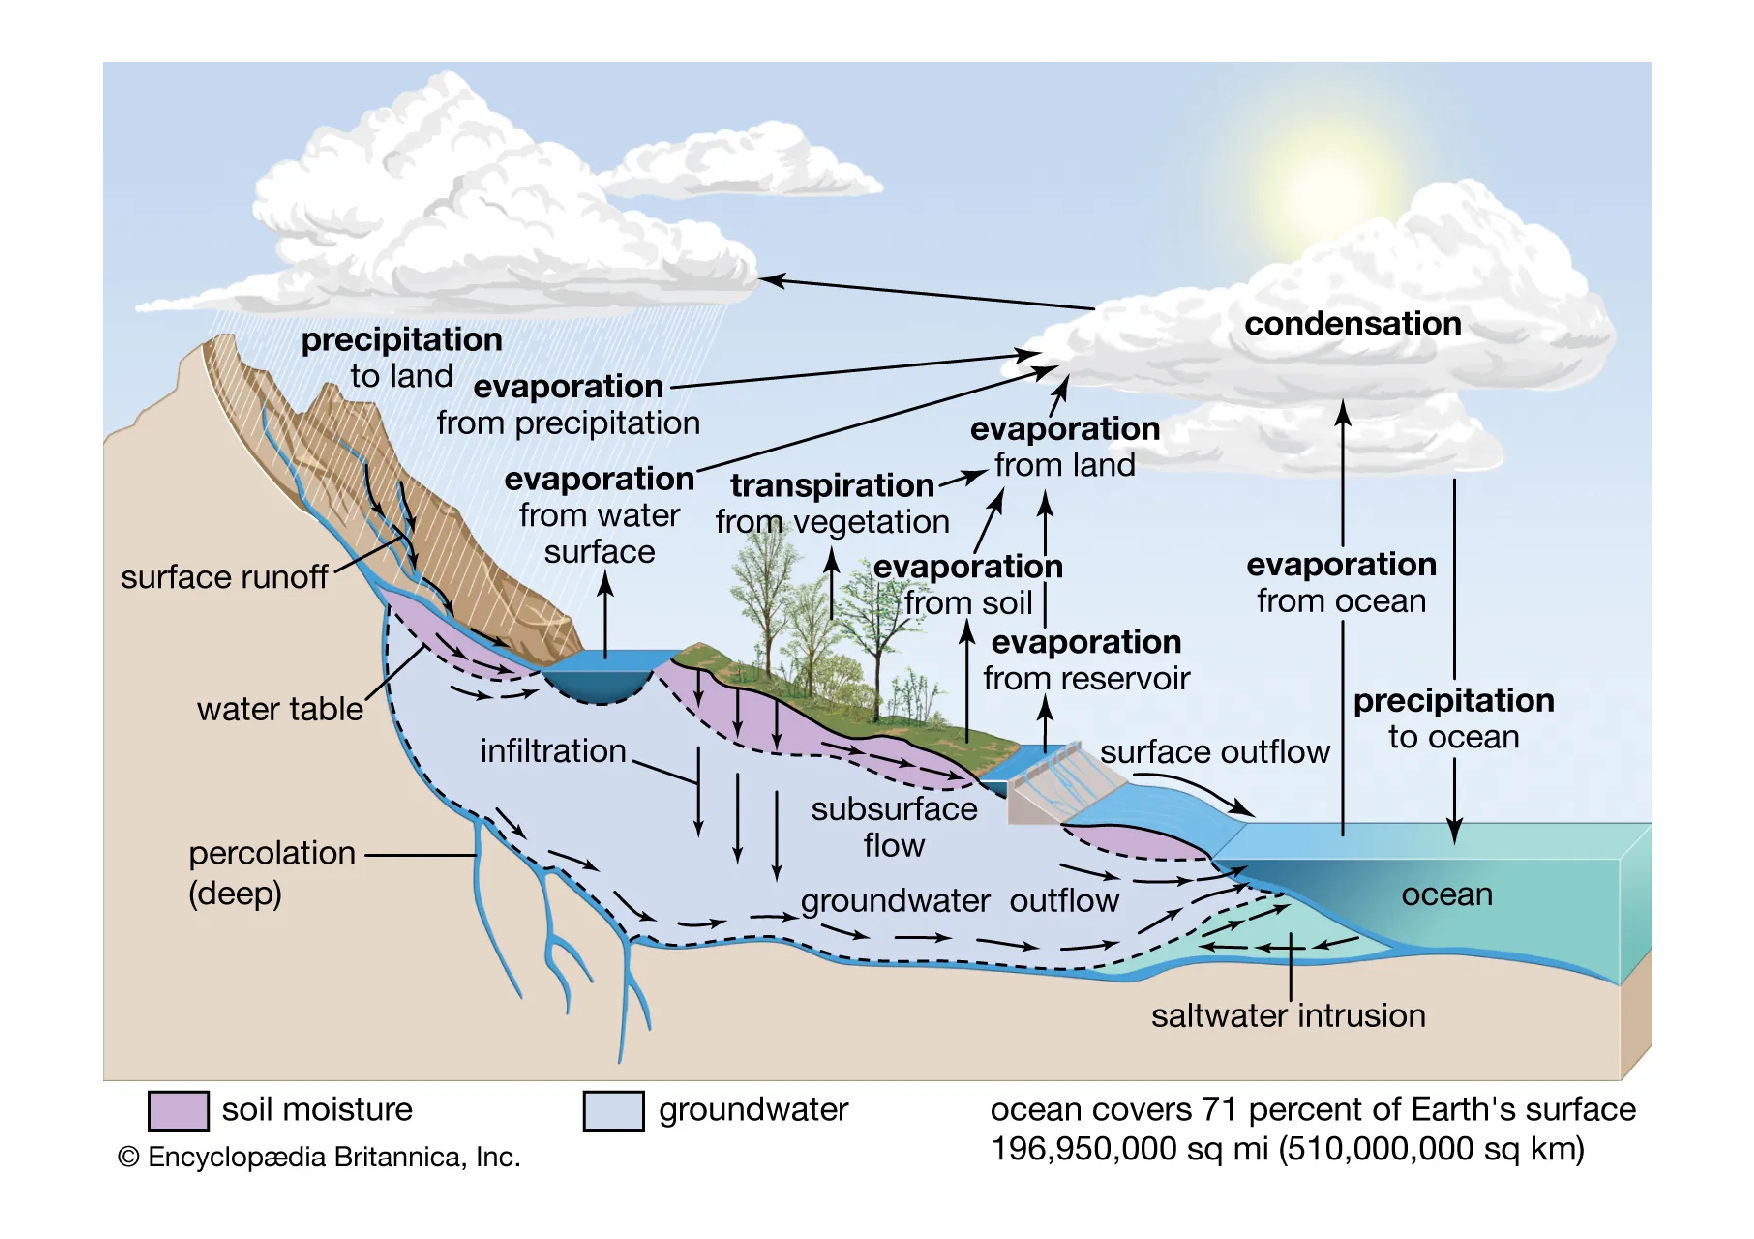
\includegraphics[width=1.0\linewidth]{Content/Figures/02_Literature_Review/hydrological-cycle.pdf}
\caption{Graphical description of the transfer of water within the hydrological cycle}
\label{fig:hydrocycle}
\end{figure}

The \textcite{EUDirective2007} addresses this issue by providing a helpful
distinction between 'flood' and 'flood risk'. Here, a flood is defined as 'a
temporary cover of land by water', while 'flood risk' is 'the combination of the
probability of a flood event and the possible adverse consequences for human
health, the environment, cultural heritage and economic activity.' This
recognition that there is a connection between social systems and the natural
environment highlights the human responsibility to find appropriate ways to
manage flood risk. \textcite{wang2022review} also provide a description of flood
risk, which shifts the perspective of floods as an 'act of god' to the idea that
the risk is constructed by societal choices to develop urban environments in
flood-prone areas. 

This definition also uses the concept of probability to describe flood risk.
Probability is a key part of flood frequency analysis (FFA), which is concerned
with predicting the likelihood of flood events of varying severity
\parencite{dalrymple1960}. Two key statistics used in FFA are Average Return
Intervals (ARIs), which describe how often a flood of a certain magnitude will
occur within a certain timeframe, and its inverse, Annual Exceedance Probability
(AEP) which gives the percentage chance of a flood of such a magnitude occurring
in any given year \parencite{Morrill2018}. Constructed using historical,
catchment-specific rainfall-runoff data, this mathematical framing of risk is
beneficial for engineering design and residual risk management purposes.
However, given that change to climatic and land-use condition can affect the
relevance of past flooding as a predictor of future flooding, the use of AEP as
a reliable flood severity metric has been questioned \parencite{Machado2015}.
AEP is used as a descriptive statistic throughout this thesis, with the
recognition that the metric can be misinterpreted within the public sphere.
Methods for managing this misinterpretation are explained later in the
literature review. AEP provides a baseline for comparing flood scenarios and
developing adaptation choices.

The intention of this thesis is to address Petone’s growing exposure to moderate
flood events due to rising relative sea levels and increased storminess
\parencite{MfE2023}. This is to be achieved by improving infrastructure
resilience, particularly through adjustments to the transport network, while
considering that a degree of residual flood risk is likely to remain even with
these improvements. To guide this goal, this thesis adopts a working definition
of flooding as follows: ‘An excess of water that surpasses the capacity of the
urban stormwater system, leading to unwanted inundation that challenges a
community’s ability to maintain essential urban functions and adapt to changing
conditions over time.’ This definition allows for flexibility and innovation in
the approaches used to manage flooding.

\subsubsection{Sources of Flooding}
It is evident from past flood events that any flood of sufficient severity has
the potential to damage interdependent infrastructure systems within urban
environments. However, several scholars have noted that making a distinction
between the source of flooding within a catchment area is critical
\parencite{White2013, chormanski2011, Pozo2023}. These distinctions influence
the design of flood defences, land-use planning, stormwater infrastructure, and
emergency response protocols. 

\textcite{Ward1978} gives attention to the physical catchment properties,
including soil type, topography, land use, and catchment size, that shape both
the causes and intensity of flooding (see figure~\ref{fig:wardfloods}).
\textcite{White2013} identifies four primary types of flooding: (1) flooding
from watercourses, (2) surface water and drains, (3) coasts and estuaries, and
(4) groundwater. These categories will be used to characterise the flood risk
landscape of the Petone-Alicetown catchment, which is exposed to multiple, often
interacting, flood hazards.

\begin{figure}
  \centering
  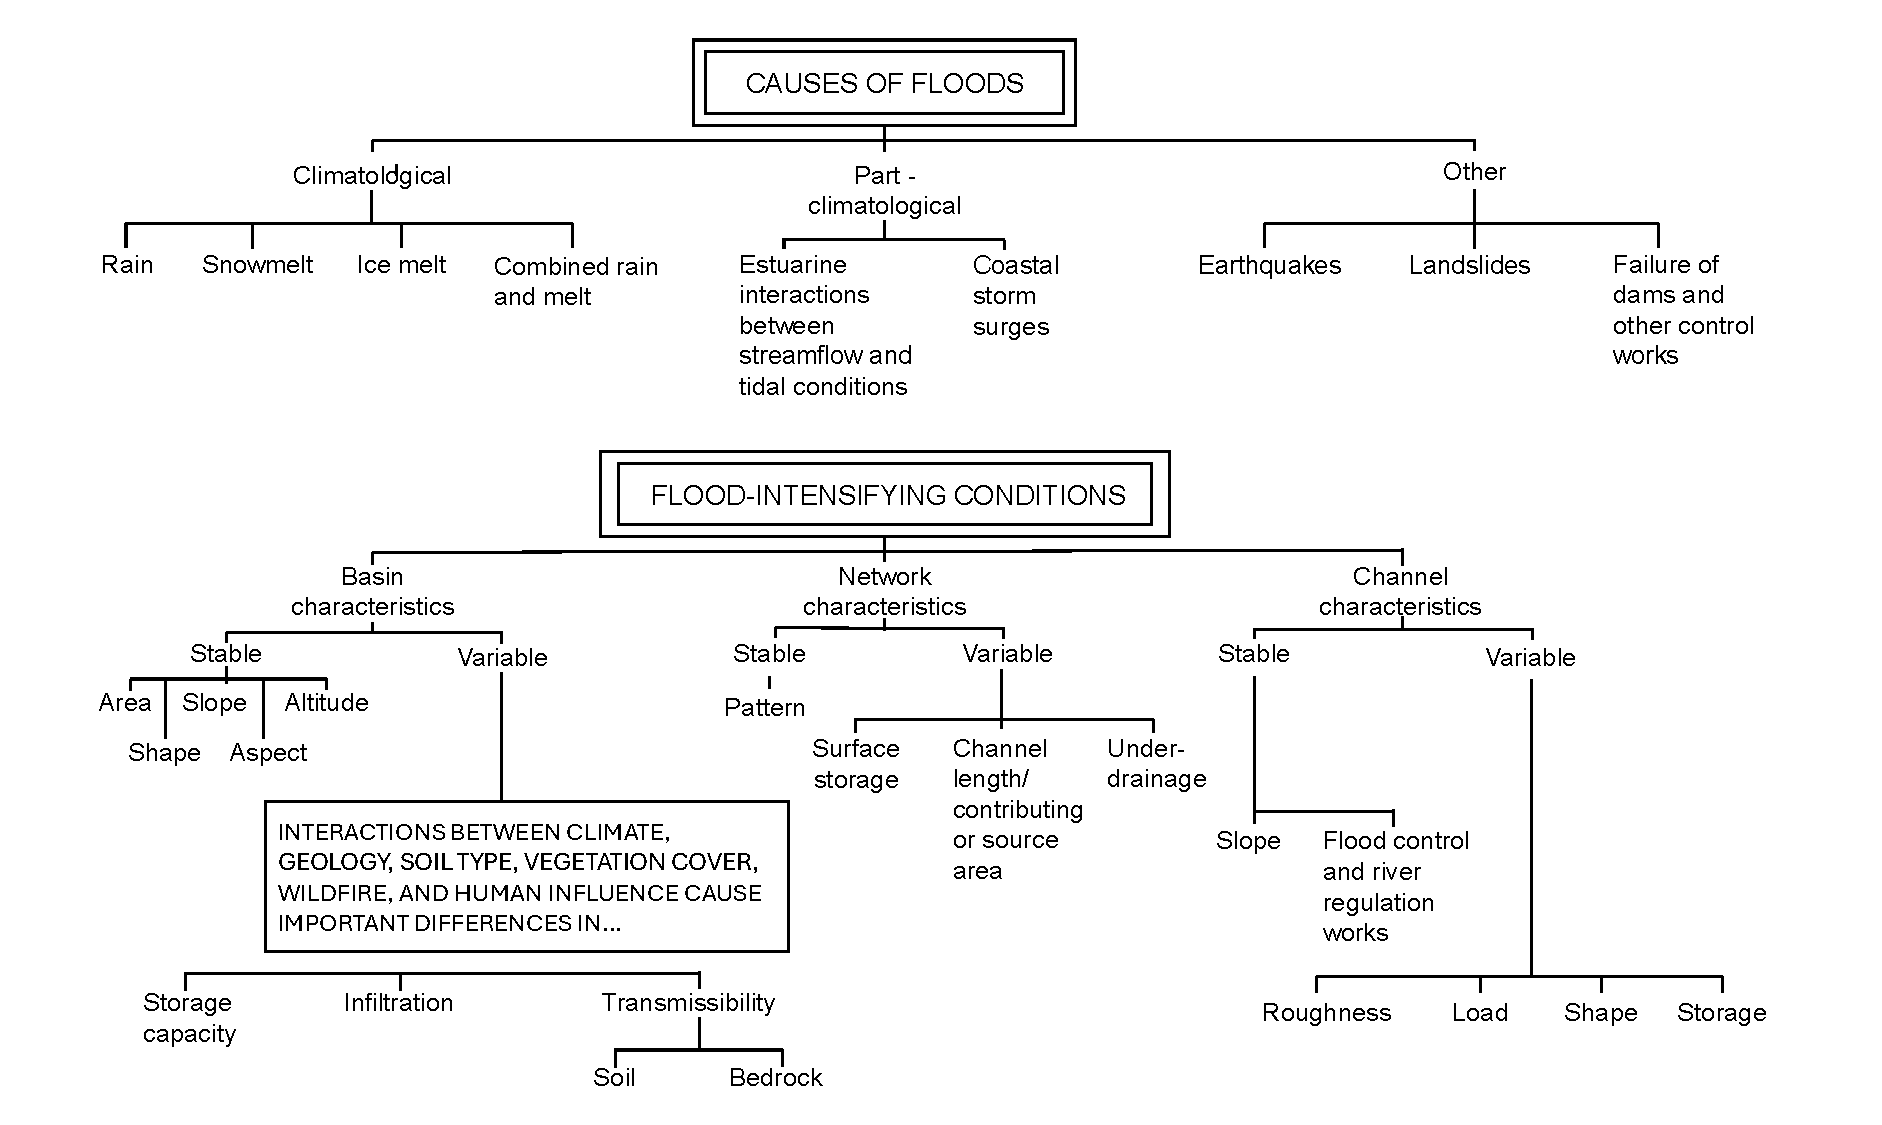
\includegraphics[width=1.0\linewidth]{02_Literature_Review/causes-of-floods}
  \caption{Causes of floods and flood-intensifying conditions as described by \textcite{Ward1978}}
  \label{fig:wardfloods}
\end{figure}

\paragraph{Flooding from Watercourses}
Watercourse, or fluvial flooding, occurs when water levels in rivers or streams
exceed the channel’s capacity, causing the overtopping of riverbanks and the
flow of flood waters into adjacent land \parencite{craig2021}. This phenomenon
can occur rapidly after intense rainfall, or more gradually due to prolonged wet
weather \parencite{smart2010}. Watercourses may be natural stream paths or
artificially constructed channels \parencite{Harding2015}, but both are
influenced by upstream rainfall, land use, channel morphology, and modifications
to riverbanks or floodplains \parencite{liu2022}.

Fluvial flood risks are a major component of New Zealand’s flood risk exposure,
in both urban and rural areas \parencite{hanna2025beyond, Fu2023}. In Petone,
the largest source of watercourse flood risk is from the Hutt River which has a
history of overtopping its banks, with particularly notable fluvial floods which
resulted in damage to residential properties and infrastructure occurring in
1898, 2009, and 2015 \parencite{ballinger2011potential, atapattu2015}. The
Korokoro stream, which crosses state highway 2, also has the potential to
inundate a major transport corridor under intense rainfall. This occurred in
1978 (see figure \ref{fig:1978flood}) and in 2015, illustrating that even minor
watercourses compromise major transportation infrastructure systems.

\begin{figure}
    \centering
    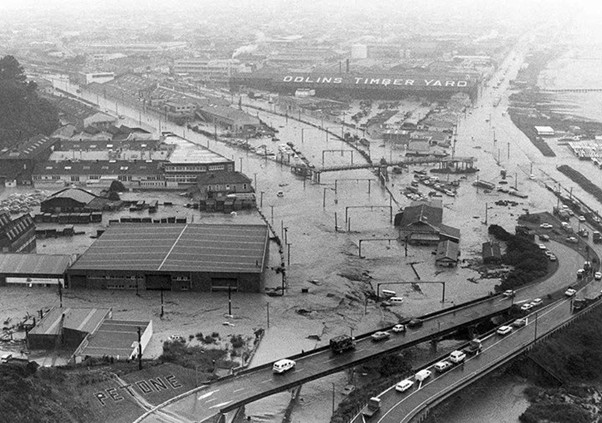
\includegraphics[width=1\linewidth]{Content/Figures/02_Literature_Review/1978flood.jpg}
    \caption{Caption}
    \label{fig:1978flood}
\end{figure}

In response to fluvial flooding, strategies such as ‘Room for the River’ and
managed retreat management options have been proposed within urban planning
schools of thought \parencite{brierley2023, lawrence2020}. However, social and
political complexity means that it is not yet known exactly how these strategies
can be executed in densely populated urban floodplains in an equitable manner
\parencite{hanna2022re, pawson2025}.

\paragraph{Flooding from Surface Water}
Surface water flooding, or pluvial flooding, typically occurs when
high-intensity rainfall overwhelms the urban stormwater system, leading to
ponding or sheet flow across impermeable surfaces \parencite{Seybert2007,
li2020}. This is distinct from river flooding in that it may occur in locations
with no existing waterways and can affect areas not traditionally mapped as
flood-prone \parencite{Pozo2023, Smart2010}.

This type of flooding is increasingly recognised as a major urban challenge due
to the prevalence of impermeable surfaces. Severe surface water flooding can
damage property and endanger people, but even shallow surface flooding of can
interfere with the day-to-day function of urban systems.
\textcite{pregnolato2017} finds that surface flood depths of 30 cm can
critically impact transport functioning, causing passenger vehicles to float.
This highlights the importance of finding ways to improve infiltration rates of
flood waters within urban areas. In Petone, surface water risk is exacerbated by
low permeability in roads and industrial areas, where runoff accumulates rapidly
during storms.

To assess these impacts, researchers have promoted the use of depth-disruption
functions that link flood depth with levels of infrastructure disruption
\parencite{kalantari2014, paulik2025}. Effective management requires increasing
infiltration and slowing runoff. While new construction on greenfield sites can
incorporate swales or permeable pavements, retrofitting older urban areas like
Petone is more complex and costly \parencite{shafique2017, WWL2022}, requiring
targeted drainage upgrades and the integration of green infrastructure where
space allows.

\paragraph{Coastal Inundation}
Coastal inundation occurs because of several, often combined meteorological and
astronomical processes which elevate sea levels to a point where low-lying
coastal margins become inundated with seawater \parencite{NIWA2023}. Changes in
mean sea level (MSL), astronomical tides, storm surge, wave setup and runup, and
the effects of climate change all influence this phenomenon (see
figure~\ref{fig:inundation}. The interaction of these drivers is non-linear and
spatially variable, meaning inundation potential differs significantly along New
Zealand’s coastlines.

\begin{figure}
    \centering
    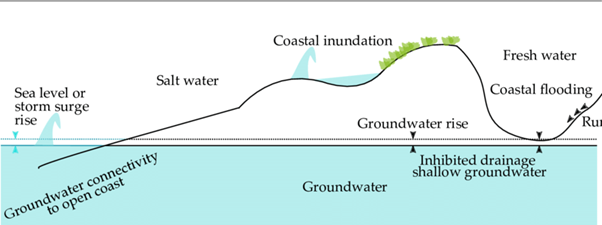
\includegraphics[width=1\linewidth]{Content/Figures/02_Literature_Review/inundation.png}
    \caption{Caption}
    \label{fig:inundation}
\end{figure}

New Zealand has a highly varied coastline with different levels of exposure to
coastal inundation. \textcite{hume2016} define 11 coastal hydrosystem
categories, which help to characterise local susceptibility to coastal flooding
(see table~\ref{table:hydrosystem}). Among the most at-risk environments are
low-lying floodplains where rivers meet the sea, such as the Hutt Valley, where
rising sea levels affect a greater land area and amplify inland flooding risks.

\begin{singlespace}
\begin{longtable}{L{5cm} L{10cm}}
\caption{Coastal hydrosystem classification for New Zealand's coastline \parencite{Hume2016}} \\
\toprule
\textbf{Geomorphic Class} & \textbf{Subclass Description} \\
\midrule
\endfirsthead

\toprule
\textbf{Geomorphic Class} & \textbf{Subclass Description} \\
\midrule
\endhead
1. Damp sand plain lake &  \\
2. Waituna-type lagoon & A. Coastal plain depression; B. valley basin. \\
3. Hāpua-type lagoon & A. Large hāpua-type lagoons; B. medium hāpua-type
lagoons; C. small hāpua-type lagoons; D. intermittent hāpua-type lagoons. \\
4. Beach stream & A. Hillside stream; B. damp-sand plain stream; C. stream with
pond; D. stream with ribbon lagoon; E. intermittent stream with ribbon lagoon.
\\
5. Freshwater river mouth & A. Unrestricted; B. deltaic; C. barrier beach
enclosed. \\
\textbf{6. Tidal river mouth} & \textbf{A. Unrestricted;} B. spit enclosed; C.
barrier beach enclosed; D. intermittent with ribbon lagoon; E. deltaic. \\
7. Tidal lagoon & A. Permanently open; B. intermittently closed. \\
8. Shallow drowned valley &  \\
9. Deep drowned valley &  \\
10. Fjord &  \\
11. Coastal embayment &  \\
\bottomrule
\end{longtable}
\end{singlespace}

The Petone foreshore experiences [relatively low tidal variation], but during
prolonged southerly winds, which are characteristic of Wellington’s climate, it
is exposed to significant wind-driven swells with inundation potential
\parencite{OPUS2010}. Even small increases in relative sea level will intensify
the magnitude and frequency of these events, reducing the return period of storm
tides that are currently considered rare.

Management strategies for coastal inundation include the construction of
seawalls, elevating infrastructure, dune restoration, and managed retreat
\parencite{Schneider2020}. However, these approaches are not without challenges.
Coastal zones are valued for their amenity and ecological function, and
proposals for structural interventions often encounter public opposition
\parencite{woodruff2018, azevedo2016}. Additionally, some scholars argue that
certain adaptive infrastructure projects can lead to maladaptation by
encouraging further development in hazard-prone areas, thereby increasing
exposure and asset value in places that remain fundamentally at risk
\parencite{logan2018, macintosh2013}.

\paragraph{Groundwater Flooding}
Groundwater flooding occurs when the water table rises to or above the surface,
causing inundation from below. Understanding the extent of groundwater flooding,
especially within urban areas \parencite{macdonald2011}, is notoriously
difficult within the discipline of hydrology \parencite{bosserelle2022,
abboud2018}. Key restrictions on the accurate prediction of groundwater flood
risk include a lack of monitoring locations, unsolved hydrological complexities,
and uncertain subsurface conditions \parencite{condon2021global}.

In low-lying coastal areas like Petone, this risk is elevated due to naturally
high groundwater tables and poorly draining soils \parencite{naish2024sea}. As
sea levels rise, the infiltration capacity of soils is reduced, increasing the
frequency and persistence of groundwater flooding \parencite{liu2020}.
Groundwater flooding may not appear as damaging as other sources of flood
waters, but it can cause significant damage to sub-surface infrastructure
systems and compromise the quality of road surfaces and building foundations
\parencite{mourot2022, bosserelle2022}. 

A high groundwater table also impedes the function of traditional gravity-based
stormwater systems \parencite{kool2020}, requiring the installation of expensive
pump-based drainage systems \parencite{WWL2022, lawrence2020}. Strategies for
managing groundwater flooding in Petone will need to be implemented over a long
time scale 

\paragraph{High Impact, Low Probability Events}

\paragraph{Compound Flooding}


\subsubsection{The Changing Nature of Flood Risk Drivers}
A major factor increasing the difficulty of flood management in urban areas is
the dynamic, changing nature of the system, both in terms of environmental and
anthropogenic change \parencite{ODonnell2020, randhir2011}. Between 1980 and
2024, the economic damage caused by flooding disasters has increased
significantly year over year, with a total cost reported in 2023 of 33.49
billion NZD (see figure~\ref{fig:damagecosts}). Some may assume that this is a
direct result of increased flood events, however the majority of researchers
consider the drivers of this increase figure to be much more complex
\parencite{Ward1978, White2013}. \textcite{White2013} discusses the four aspects
of the changing world that may be contributing to an increase in natural
disasters being reported: (1) there is a rise in severity of natural weather
patterns, (2) societies may play a role in amplifying the hazard, (3) people are
increasingly exposed to risks from extreme events, and (4) people are more
vulnerable to experiencing the effects. 

\begin{figure}
    \centering
    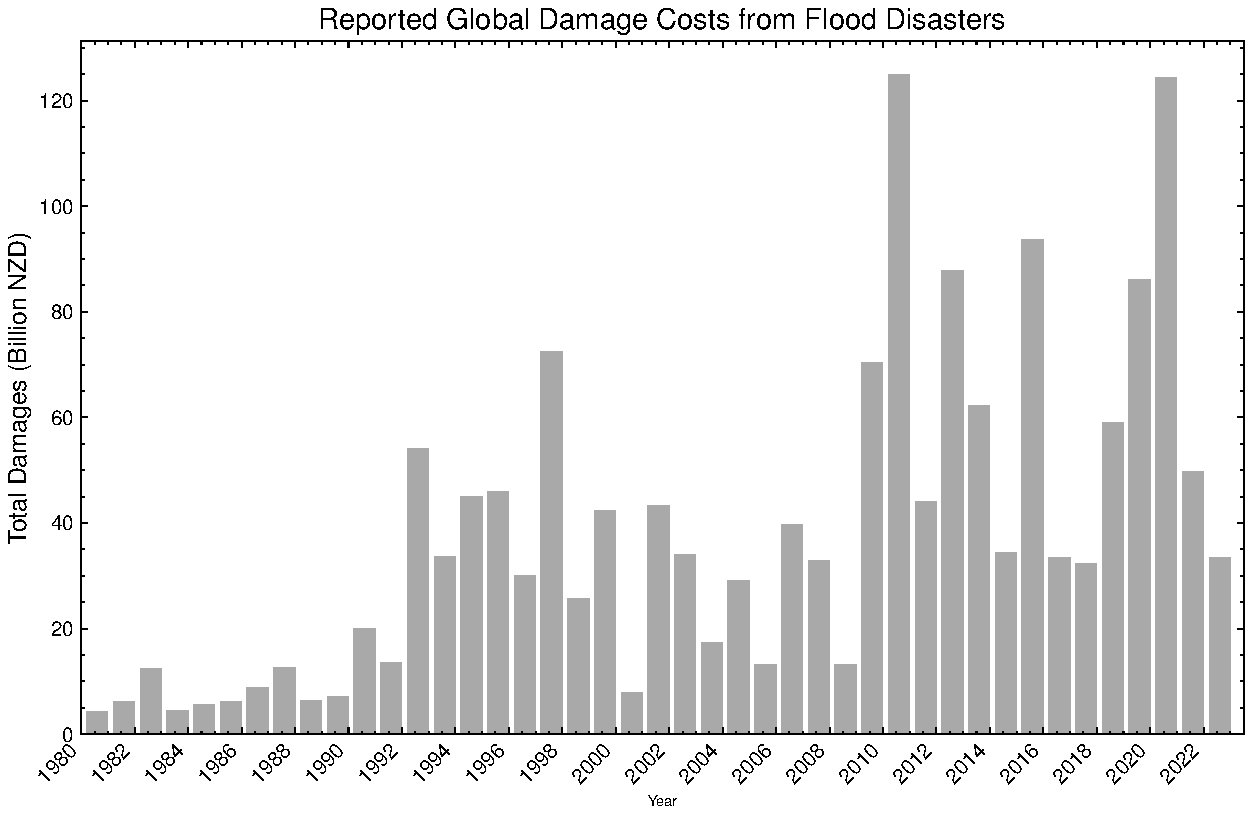
\includegraphics[width=1.0\linewidth]{Content/Figures/02_Literature_Review/damage_costs_natural_disasters}
    \caption{An increase in the global reported costs of damage resulting from flooding over the last 35 years.}
    \label{fig:damagecosts}
\end{figure}

\paragraph{Climatic and Environmental Drivers}
\begin{figure} % Requires \usepackage{float}
  \centering
  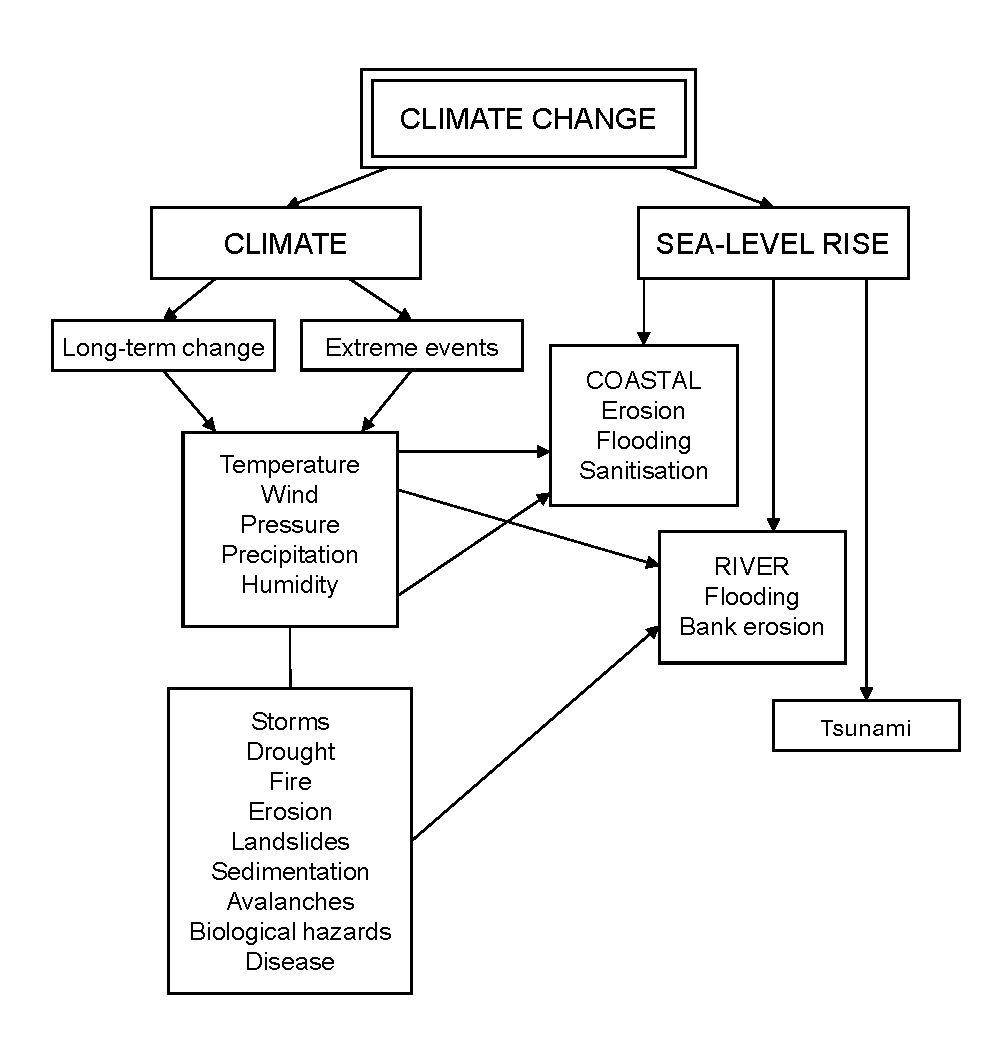
\includegraphics[width=0.9\linewidth]{02_Literature_Review/Hazards}
  \vspace{-1em}
  \caption{Overview of increased hazards due to climate change, adapted from Pickering and Owen, 1997 (p.149)}
  \label{fig:hazards}
\end{figure}


\begin{singlespace}
\begin{longtable}{L{2.5cm} L{3cm} L{8cm}} \caption{Excerpt of Table 1 in
O'Donnell (2018). S = Source, P = Pathway, R = Receptor. \textsuperscript{a} =
Recent additions to Evans et al. (2008)} \\
\toprule
\textbf{Driver Group} & \textbf{Driver} & \textbf{Explanation} \\
\midrule
\endfirsthead

\toprule
\textbf{Driver Group} & \textbf{Driver} & \textbf{Explanation} \\
\midrule
\endhead

% Your table content here
Climate change (S) & Precipitation & changes in short-duration precipitation—amount, intensity, duration, location, seasonality and clustering \\
                   & Temperature & influence of temperature on soil moisture and
                   hence runoff. \\
                   & Relative sea-level rise & Rising relative sea level due to climate change-induced melting of icecaps and thermal expansion in conjunction with land subsidence or uplift. Makes coastal flooding more frequent. \\
                   & Waves & increases in the height and direction of coastal waves will transmit more wave energy to the shoreline at some locations and less energy at others, increasing the risks that waves will breach and overtop coastal defences. \\
                   & Storm surges & increases in surge levels are expected due to climate change-induced increases in storminess. Stronger surges mean that higher extreme water levels with more energy reach the shoreline, increasing risks of breaching or overtopping of coastal defences. \\
\midrule
Catchment runoff (P) & Urbanisation & a change in land management with green field and previous surfaces covered by less pervious materials (buildings and infrastructure) and associated new conveyance systems. \\
\midrule
Groundwater systems and processes (P) & Groundwater flooding & groundwater flooding occurs when the water table reaches the elevation of the land surface (waterlogging) or by the emergence of water originating from subsurface permeable strata. \\
\midrule
Fluvial systems and processes (P) & River morphology and sediment supply & changes in river channel morphology (size and shape) and sediment supply that alter attributes of the river channel and floodplain to influence flood conveyance, routing and storage. \\
\midrule
Urban systems and processes (P) & loss of floodable urban spaces\textsuperscript{a} & loss of urban spaces that previously helped reduce flood risk through infiltration, attenuation or storage. Includes the loss of urban green space and brownfield land (to buildings and infrastructure) and changes in the types of urban green space that affect its rainfall-runoff reduction potential. \\
\midrule
Coastal processes (P) & Coastal morphology and sediment supply & changes in the near shore sea-bed, shoreline and adjacent coastal land, coastal inlets and estuaries will in the short term affect the wave and surge energies that affect the shoreline. \\
\midrule
Human behaviour (P) & Stakeholder behaviour & the behaviour of individuals, groups and institutions will influence flood risk. Different mechanisms will accommodate different stakeholders' interests. \\
\midrule
Socio-economics (R) & Infrastructure Impacts & the relationship between flood risks and the array of networks and nodes that deliver physical services including gas, water, electricity, transport, telecoms, etc. \\
                    & Indirect economic impacts\textsuperscript{a} & the indirect impacts of flood events including losses from capital and labour productivity disruptions, e.g. flooded roads interrupting transportation and consequentially disrupting economic activities \\
\bottomrule
\end{longtable}
\end{singlespace}

\paragraph{Climate and Environmental Drivers}

The nature and occurrence of a flood is highly dependent on environmental
conditions. textcite{Ward1978} separates the relevant flood drivers into 'causes
of floods' and 'flood-intensifying conditions'. Enviornmental factors are a
direct cause of flooding, Coastal environments are particularly susceptible to a
range of environmental hazards including relative sea level rise, Coastal
environments are uniquely exposed to a multitude of environmental phenomena,
including The key phenomena discussed below, including increasing atmospheric
moisture, 

\paragraph{Anthropogenic Drivers}

Anthropogenic drivers are undoubtedly impacting the climate, and hence the
environmental drivers of flooding, but 

- Urbanisation
- Upstream Land Use Change
- Population Growth and Land Pressure
- Infrastructure Development

\subsubsection{Modelling Floods}

\subsection{Building Resilience to Floods}

\subsubsection{Defining Resilience}

\subsubsection{Structural Interventions}

\paragraph{Critical Infrastructure}

\paragraph{Transport Infrastructure}

\paragraph{Implementing Resilient Infrastructure}

\subsubsection{Non-Structural Interventions}

\begin{figure}
    \centering
    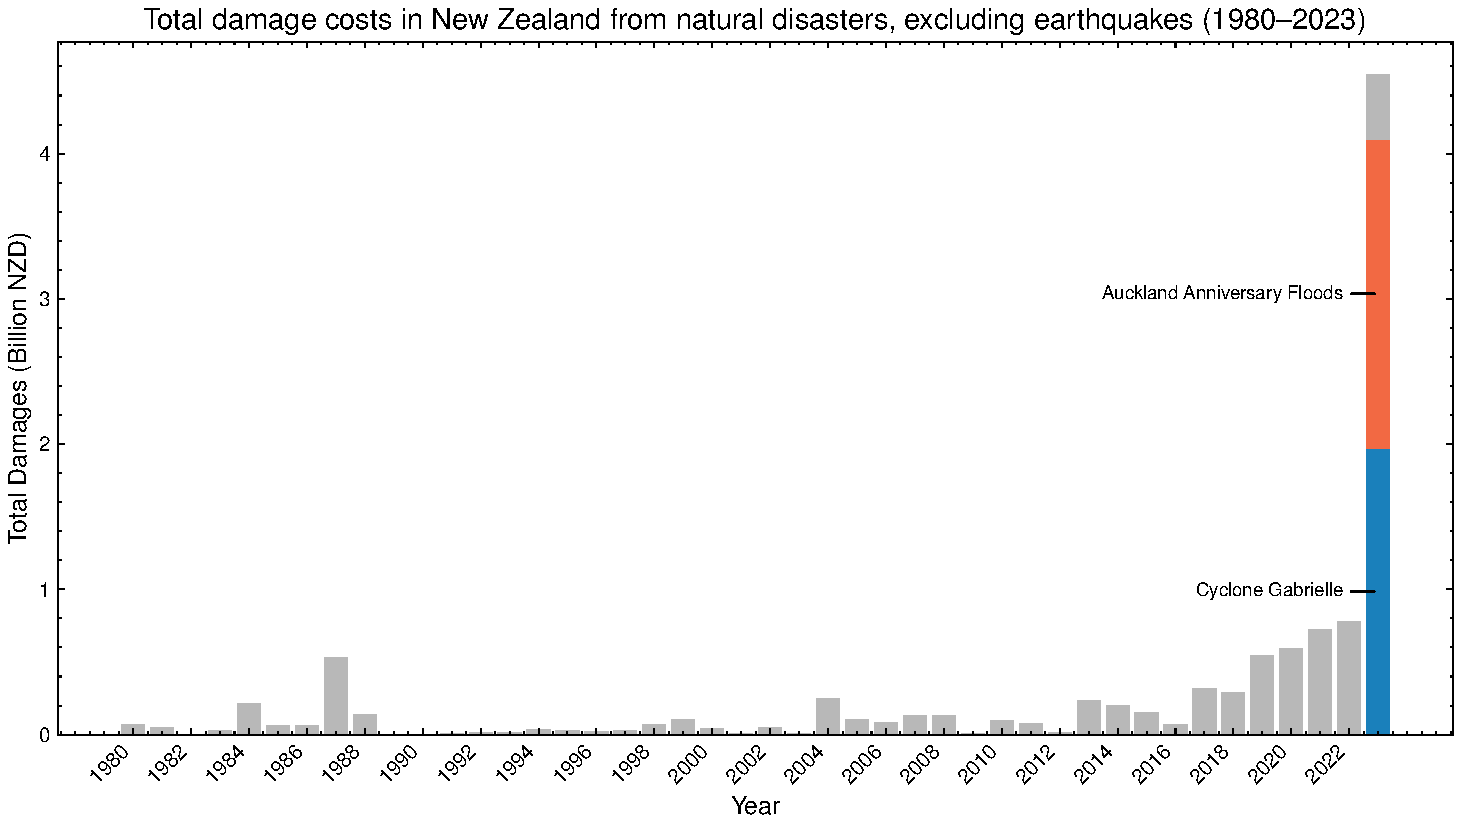
\includegraphics[width=1.0]{Content/Figures/02_Literature_Review/damage_costs_NZ_natural_disasters.pdf}
    \caption{Natural disasters include: cyclones, extreme weather, flooding, fires, landslides.}
\end{figure}
\subsection{Nature-based Solutions for Urban Flood Resilience}

\subsubsection{Defining Nature-based Solutions}

\subsubsection{Achieving Urban Flood Resilience with NBS}

\subsubsection{NBS Design Typologies}

\paragraph{Rain Gardens}

\paragraph{Swales and Filter Strips}

\paragraph{Dry Retention Basins}

\paragraph{Coastal NBS}

\subsubsection{Co-Benefits of NBS}

\subsubsection{Facilitating the Uptake of NBS}

\paragraph{Competition for Space}

\paragraph{Perceived Costs}

\paragraph{Retrofitting NBS into Urban Environments}

\paragraph{Maintenance Responsibilities}

\subsection{Planning Under Uncertainty}

\subsubsection{Sources of Uncertainty}

\subsubsection{Dynamic Adaptive Pathways Planning}

\subsubsection{Decision Tools}
\section{Methodology}
\subsection{GIS-based Risk Assessment}

\subsection{Adaptation Option Development}

\subsection{Cost-Benefit Analysis}

\section{Results}
\input{Content/Body_Text/04_Results}
\section{Discussion}
\input{Content/Body_Text/05_Discussion}
\section{Conclusion}
\input{Content/Body_Text/06_Conclusion}
%================= BIBLIOGRAPHY ==================%
\newpage
\printbibliography{}

\end{document}

